\documentclass[12pt]{article}
\usepackage{graphicx,hyperref,fancyvrb}
\begin{document}
\title{Using Dynamic Anaylsis Tools}
\author{David W. Juedes}

\maketitle
\section{Introduction: Why should I care?}
This brief document discusses dynamic analysis tools that are
available to Computer Science (and Computer Engineering) students at Ohio
University.  In this document, I will discuss how to use them, and why you might want to use them.   The answer to why you might want to use them 
is somewhat simple: using dynamic analysis tools makes coding much
faster because it makes finding bugs much, much easier.  This is especially 
true for programming languages like C++ that will continue to execute even if the program performs apparently incorrect statements 
(e.g., accessing an array out of bounds, or dereferencing an 
uninitialized pointer).  Dynamic analysis tools are less important for programming languages such as Java, where those same apparently incorrect statements would generate an exception.
 
I am writing this brief document because I believe that every student
who is taking a CS course higher than 240A should be aware of dynamic
analysis tools and understand how to use them to make software
development more efficient.  I strongly suggest that any student in CS
240B to read this document carefully.  It will make your life a lot
easier.

\section{Static vs. Dynamic Analysis}
The term \emph{static analysis} refers to a collection of techniques
that can be used to examine what might happen when source code is
executed by simply examining the source code itself.  Static analysis
have been around for at least 40 years.  The UNIX program \verb+lint+
was an excellent, early example of a program that performed static
analysis of source code.  Now, most compilers have a fair bit of
static analysis built in, such as the GNU C/C++ compiler.   
\vspace*{0.2 in}

\noindent \framebox[\textwidth]{\parbox{\textwidth}{Programming Tip \#1: Always compile your code using the 
{\tt gcc/g++ -Wall} flag.  This will perform static analysis on your code and 
tell you if there are any obvious problems.   Some problems can be ignored, but, as a general rule thumb it is good to fix any error detected by the {\tt -Wall} flag.}}
\vspace*{0.2 in}


In contrast, the term \emph{dynamic analysis} refers to a collection
of techniques that can be used to examine what happens when source
code is executed.  These techniques typically involve simulating the
program in a way that enables fine-grained memory analysis.  Such a
fine-grained memory analyses can detect (i) array out-of-bounds
errors, (ii) branches (if's, etc.) on uninitialized variables, (iii)
pointer problems, (iv) memory leaks, and other similar errors.  
These types of errors can sometimes cause fatal problems 
much later on in a program's execution.  But, a program may have one or
more of these types of error and still execute correctly (i.e., it may pass
every test case).  Since such errors may or may not exhibit 
noticable effects, they can be very tricky to detect.  

In this brief document, I will discuss two dynamic analysis tools: {\tt discover
} which runs on the Sun Workstations in Stocker Center, and {\tt valgrind} which runs under most versions of Linux.  There are other available dynamic analysis tools.   A good survey of these tools can be found on the appropriate 
wiki page: \href{http://en.wikipedia.org/wiki/Dynamic_program_analysis}{Dynamic Program Analysis}
\vspace*{0.2 in}

\noindent \framebox[\textwidth]{\parbox{\textwidth}{Programming Tip \#2: 
Find a good dynamic analysis tool and use it frequently.}}
\vspace*{0.2 in}

\section{Four Example Programs}
To begin, let's look at four example programs that have errors.
\subsection{Test.cc}
We named the first one \verb+test.cc+.  Can you see the bugs?

\begin{Verbatim}[numbers=left,frame=single]
//******************************
//* A simple C++ program with several bugs.
//* The bugs are easy to find with DISCOVER.
//*
//********************************************** 
#include <vector>
#include <iostream>
using namespace std;
int main() {
   vector<int> vec;
   vec.resize(10);
   for (int i=0;i<=10;i++) {
      vec[i] = i;
   }
   int sum;
   for (int i=0;i<=10;i++) {
       sum+=vec[i];
   }
   cout << sum << endl;
}
\end{Verbatim}

This program runs correctly and gives the correct answer 55 ($\sum\limits_{i=0}^{10} i = 55$)

\subsection{Test1.cc}
We named the second program \verb+test1.cc+.

\begin{Verbatim}[numbers=left,frame=single]
#include <iostream>
using namespace std;
void foo(bool x) {
  if (x) {
    cout << "This worked" << endl;
  } else {
    cout << "Oops this didn't work "<< endl;
  }
}
int main() {
  bool test;
  foo(test);
}
\end{Verbatim}
This program runs and prints ``Oops this didn't work.''
What's wrong here?
\subsection{Test2.cc}
We named the third program \verb+test2.cc+.
\begin{Verbatim}[numbers=left,frame=single]
/* This one does something bad....
   Guess what it is.   */
#include <iostream>
#include <cstdlib>

using namespace std;

int main() {

  int *x;

  x = NULL;

  x[0] = 10;

}
\end{Verbatim}
This program generates the run-time error: \verb+Segmentation fault (core dumped)+.
Can you see what is wrong?

\subsection{Test3.cc}
We named the fourth program \verb+test3.cc+.
\begin{Verbatim}[numbers=left,frame=single]
#include <iostream>

using namespace std;

int foo(bool x) {
  if (x) {
    cout << "This worked" << endl;
  } else {
    cout << "Oops this didn't work "<< endl;
  }

}
int main() {

  bool test=true;

  cout << foo(test) << endl;
}
\end{Verbatim}
Can you see the problem here?


Now, it does not matter whether you can see what is wrong with these 
simple programs because a good dynamic analysis tool can point out 
the errors right away. 

Let's look at what \verb+discover+ and \verb+valgrind+ say about these four programs.

\section{It pays to use ``{\tt discover}''}
In order to use \verb+discover+ to find errors, you must 
(i) first compile your code correctly , (ii) ``instrument'' your code using 
the discover command, and (iii) run the instrumented version of your code.
When you complete step (iii), the instrumented code will generate a report that
describes all of the errors that it found.

The \verb+discover+ command works best with SUN C++ compiler (CC).  This compiler
is located in the directory \verb+/opt/opt/solstudioex1006/bin+.  So, to
perform step (i), you must issue a command like:
\begin{verbatim}
/opt/solstudioex1006/bin/CC -g -O2 test.cc
\end{verbatim}
(If that directory is in your path, then \verb+CC -g -O2 test.cc+ should work as well.)
According to the man page for CC, the \verb+-g+ option tells the compiler to ``prepare the executable for debugging.''  The \verb+-O2+ limits the number
of optimizations the compiler makes.  To perform step (ii), issue the
discover command as follows:
\begin{verbatim}
/opt/solstudioex1006/bin/discover -o test.disc a.out
\end{verbatim}
This creates a new executable called \verb+test.disc+.  You can then run this
executable, just like you'd run \verb+a.out+:
\begin{verbatim}
./test.disc
\end{verbatim}
However, once you run \verb+test.disc+, it will not only execute the program, but
it also writes a report.  The default report is placed in the file
\verb+[executable].html+, which in this case is \verb+test.disc.html+.
To see the output of discover, open this file inside of a web-browser (Select File $>$ Open File on the menu.)   
\vspace*{0.2 in}

\noindent \framebox[\textwidth]{\parbox{\textwidth}{Programming Tip \#3: 
You can have {\tt discover} produce its output directly to the terminal.  To do this, execute the command {\tt discover -w - -o test.disc a.out} instead of the one given above.  In this case, the {\tt -w} flag tells discover where 
to write the output.  Usually, this would be a file name, but, in this 
case, the {\tt -} indicates the standard output (terminal) instead of a file.}}
\vspace*{0.2 in}


Now, let's look at the output of \verb+discover+ on the four programs.

\subsection{Discover on Test.cc}
For \verb+test.cc+, the output of \verb+discover+ looks as follows:
(Make sure to click on ``Show'' under ``All Details'' and ``All Source'' on the menu on the left to get this view.)
\begin{center}
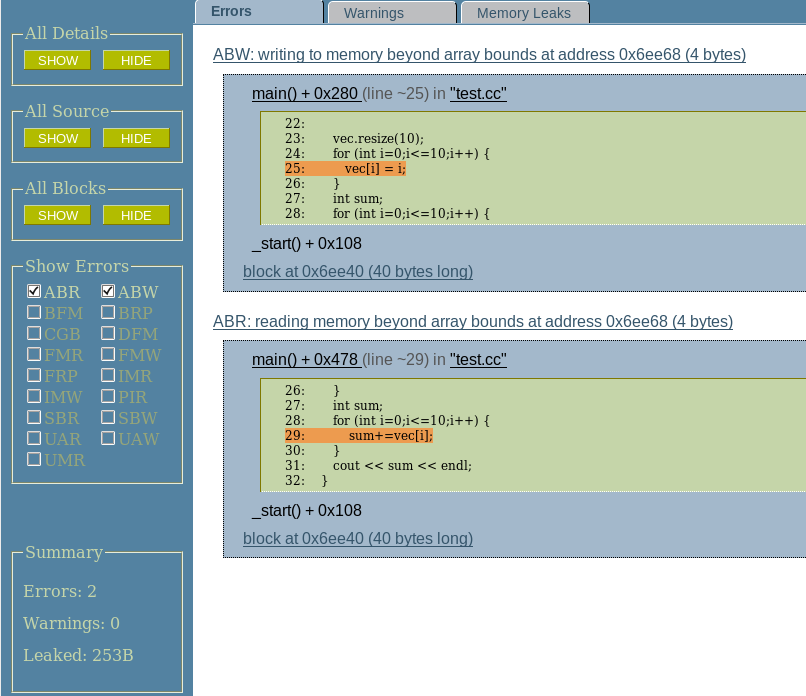
\includegraphics[width=6 in]{images/test.png}
\end{center}

For this program, a simple visual inspection of the program reveals that
the vector \verb+vec+ was created with 10 elements (0..9).  The 
two for-loops access element \verb+10+ in the vector, which is outside the stated range of the dynamic array. 

\subsection{Discover on Test1.cc}
Running discover, as described above, on \verb+test1.cc+ 
gives the following output.
 
\begin{center}
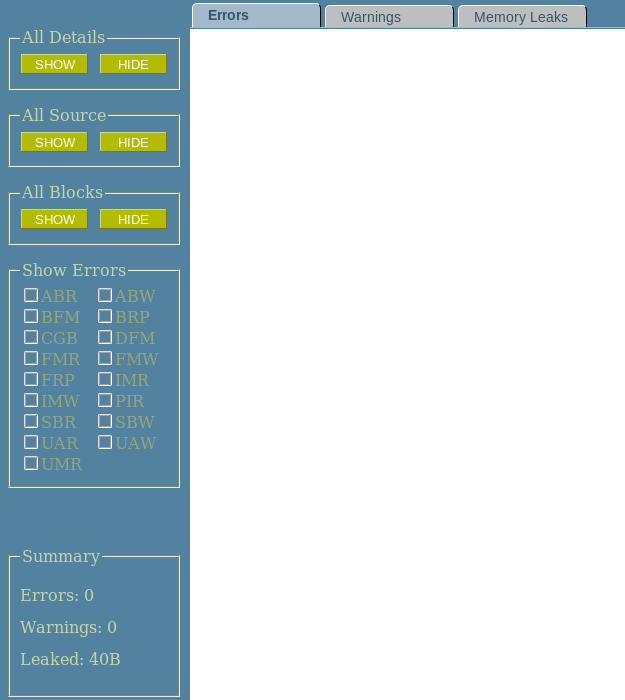
\includegraphics[width=6 in]{images/test1.png}
\end{center}

Notice that no errors were discovered.  It should be pointed out that
the compiler provides the appropriate error message in this case: the variable \verb+test+ is uninitialized.

\subsection{Discover on Test2.cc}
Running discover, as described above, on \verb+test2.cc+ 
gives the following output.

\begin{center}
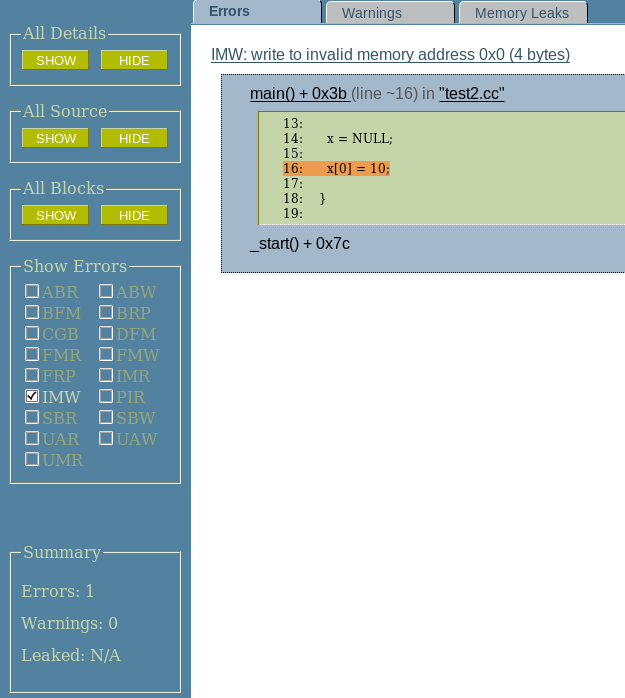
\includegraphics[width=5 in]{images/test2.png}
\end{center}

In this case, setting the pointer variable \verb+x+ to NULL causes the
the array assignment \verb+x[0]=10;+ to write the value 10 to an 
invalid memory address.

\subsection{Discover on Test3.cc}
The output of discover for \verb+test3.cc+ is as follows.
\begin{center}
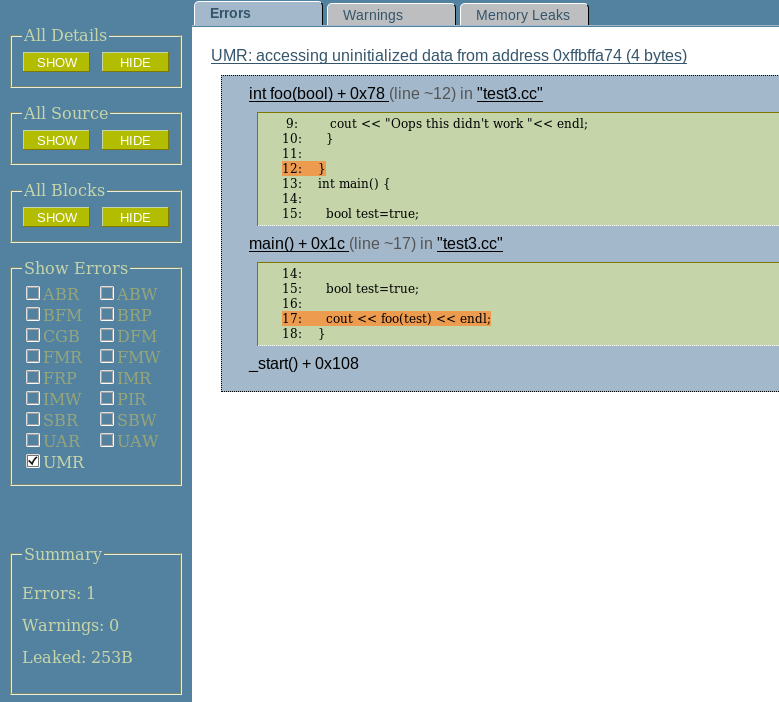
\includegraphics[width=5 in]{images/test3.png}
\end{center}

Notice that the error occurs when the function \verb+foo+ is
executed.   If you examine the code, you will notice that
\verb+foo+ does not return a value.   This will cause severe problems
if not addressed.

\section{Using {\tt valgrind} }
If you use Linux (Ubuntu, Redhat, etc.), you will probably use \verb+valgrind+
instead of \verb+discover+.  Both programs do the same things, in slightly different ways.

\subsection{Using {\tt valgrind}}
As mentioned in the valgrind man page:
\begin{quote}
Valgrind is a flexible program for debugging and profiling Linux
executables. It consists of a core, which provides a synthetic CPU in
software, and a series of debugging and profiling tools. The
architecture is modular, so that new tools can be created easily and
without disturbing the existing structure.
\end{quote}
In order to use \verb+valgrind+, you must first compile your program
with the same flags you would use for debugging, i.e., \verb+-g+.
In the case of \verb+test.cc+, we would compile the program
as follows:
\begin{verbatim}
g++ -g  -O2 test.cc
\end{verbatim}
This creates the executable \verb+a.out+. 
Now, to run \verb+valgrind+, we issue the \verb+valgrind+ command as follows:
\begin{verbatim}
valgrind a.out
\end{verbatim}
In the case of \verb+test.cc+, the output of valgrind is the
following.
{\small
\begin{verbatim}
==5309== Memcheck, a memory error detector
==5309== Copyright (C) 2002-2009, and GNU GPL'd, by Julian Seward et al.
==5309== Using Valgrind-3.5.0 and LibVEX; rerun with -h for copyright info
==5309== Command: a.out
==5309== 
==5309== Invalid write of size 4
==5309==    at 0x8048891: main (test.cc:24)
==5309==  Address 0x4025050 is 0 bytes after a block of size 40 alloc'd
==5309==    at 0x4006350: operator new(unsigned int) (vg_replace_malloc.c:214)
==5309==    by 0x8048AC1: std::vector<int, std::allocator<int> >::
_M_fill_insert(__gnu_cxx::__normal_iterator<int*, std::vector<int, 
std::allocator<int> > >, unsigned int, int const&) (new_allocator.h:89)
==5309==    by 0x804887E: main (stl_vector.h:851)
==5309== 
==5309== Invalid read of size 4
==5309==    at 0x80488A1: main (test.cc:28)
==5309==  Address 0x4025050 is 0 bytes after a block of size 40 alloc'd
==5309==    at 0x4006350: operator new(unsigned int) (vg_replace_malloc.c:214)
==5309==    by 0x8048AC1: std::vector<int, std::allocator<int> >::
_M_fill_insert(__gnu_cxx::__normal_iterator<int*, std::vector<int, 
std::allocator<int> > >, unsigned int, int const&) (new_allocator.h:89)
==5309==    by 0x804887E: main (stl_vector.h:851)
==5309== 
7614507
==5309== 
==5309== HEAP SUMMARY:
==5309==     in use at exit: 0 bytes in 0 blocks
==5309==   total heap usage: 1 allocs, 1 frees, 40 bytes allocated
==5309== 
==5309== All heap blocks were freed -- no leaks are possible
==5309== 
==5309== For counts of detected and suppressed errors, rerun with: -v
==5309== ERROR SUMMARY: 2 errors from 2 contexts (suppressed: 16 from 9)
\end{verbatim}
The important lines in the above output are:
\begin{verbatim}
==5192== Invalid write of size 4
==5192==    at 0x80488C9: main (test.cc:25)
==5192== Invalid read of size 4
==5192==    at 0x80488FA: main (test.cc:29)
\end{verbatim}
These lines correspond to
\begin{verbatim}
25:      vec[i] = i;
\end{verbatim}
and
\begin{verbatim}
29:      sum+=vec[i];
\end{verbatim}
Again, as mentioned above, these errors are caused because the vector
has been allocated to have 10 elements (0..9), but the 10th element
has been read and written to.   As with most compilers/debuggers, it
is best to fix the first errors, and then rerun valgrind.  Changing 
line 23 to:
\begin{verbatim}
vec.resize(11);
\end{verbatim}
recompiling and rerunning valgrind gives the following output.
{\small 
\begin{verbatim}
==5336== Memcheck, a memory error detector
==5336== Copyright (C) 2002-2009, and GNU GPL'd, by Julian Seward et al.
==5336== Using Valgrind-3.5.0 and LibVEX; rerun with -h for copyright info
==5336== Command: a.out
==5336== 
7614507
==5336== 
==5336== HEAP SUMMARY:
==5336==     in use at exit: 0 bytes in 0 blocks
==5336==   total heap usage: 1 allocs, 1 frees, 44 bytes allocated
==5336== 
==5336== All heap blocks were freed -- no leaks are possible
==5336== 
==5336== For counts of detected and suppressed errors, rerun with: -v
==5336== ERROR SUMMARY: 0 errors from 0 contexts (suppressed: 16 from 9)
\end{verbatim}}
\vspace*{0.2 in}

\noindent \framebox[\textwidth]{\parbox{\textwidth}{Programming Tip \#4:
Always fix the first error that you discover using a dynamic analysis
tool and then retest.  Sometimes, errors cascade.  Hence, one error may
result in many errors being reported in any dynamic analysis tool.}}
\vspace*{0.2 in}

\noindent \framebox[\textwidth]{\parbox{\textwidth}{Programming Tip \#5:
When using dynamic analysis tools, remember to compile your program
using the optimization flags {\tt -g -O2}.  If you forget the 
{\tt -O2} flag, the compiler may use optimizations that are not
compatible with {\tt valgrind} or {\tt discover}.}}
\vspace*{0.2 in}

%%%
% Latex Hack to use verbatim inside of a BOX.
% This probably also works with footnotes!
%
\newsavebox{\mybox}
\begin{lrbox}{\mybox}
\verb+valgrind a.out &>val.out+
\end{lrbox}


\noindent \framebox[\textwidth]{\parbox{\textwidth}{Programming Tip \#6:
When using valgrind, save the output as follows:
\usebox{\mybox}.
Then, look for errors related to the files that you created (e.g., test3.cc) using a text editor.  Ignore all other errors. }}
%}
\vspace*{0.2 in}



\noindent \framebox[\textwidth]{\parbox{\textwidth}{Exercise \#1:
Use {\tt valgrind} to try to discover the errors in test1.cc, test2.cc, and test3.cc.}}
\vspace*{0.2 in}

Notice that valgrind actually supports a number of tools (memcheck -- default, 
cachegrind, etc.).  Also, notice that there is a patch to 
gcc (but not g++) that allows for bounds checking for objects
allocated to the stack.  See \href{http://sourceforge.net/projects/boundschecking/}{here} for more details. 


\end{document}
